\section{Design}
\subsection{Type checking background}
The major components of a type system include: 1) \textit{types}, 2) \textit{subtyping rules}, and 3) \textit{dataflow analysis}.
A \textit{type} serves as an abstraction for the set of acceptable values for any expression. The types in a type system form a lattice of finite height. 
The hierarchy of types in this lattice defines subtyping relationships among them.
In our framework, we require every type hierarchy to define a unique\<@Top> and a \<@Bottom> element. This ensures that
any given pair of types has a \textit{least upper bound} and a \textit{greatest lower bound}.
Throughout this paper, we use the notation \<@A> <: \<@B> to denote that type \<@A> is a subtype of type \<@B>.
As an illustration of the type hierarchy, consider the lattice of types shown in Figure~\ref{fig-example-lattice}.
\begin{figure}
	\begin{center}
		\includegraphics[scale=0.15]{lattice}
	\end{center}
	\caption{Example type hierarchy}
	\label{fig-example-lattice}
\end{figure}
In this type system, \<@C> is a subtype of \<@A> as well as \<@B> and types \<@A> and \<@B> are incomparable.
The type checker now performs additional type checking (similar to javac's type checking) with respect to this type hierarchy
and reports any violations. The snippet in Figure~\ref{code-invalid1} would result in an error at the assignment statements:
\begin{figure}
	\begin{verbatim}
	@A int x; @B int y; @C int z;
	x = y;    // Because types @A and @B are incomparable.
	z = x;    // Because @C is a subtype of @A.
	\end{verbatim}
\caption{Example: Invalid assingment}
\label{code-invalid1}
\end{figure}

Similarly, if the return type of a method is annotated as \<@C> but it returns a type that has either \<@A> or \<@B>, the
checker would report an error at compile time.

%Method overriding and example
For method overriding, the usual rules apply for parameters and arguments i.e covariant subtyping for parameters
and contravariant subtyping for return types. Consider the example in Figure~\ref{code-invalid2} where method \<foo> of \<class X> is overridden
in \<class Y>.
\begin{figure}
	\begin{verbatim}
	class X {
	    @B int foo(@C int param) {}
	}
	class Y extends X {
	    @C int foo(@B int param) {}
	}
	\end{verbatim}
	\caption{Example: Invalid Method override}
	\label{code-invalid2}
\end{figure}

The overriding method is invalid for two reasons: type of the parameter (\<@B>) is not a subtype of the parameter type in the overriden method (\<@C>) and the return type (\<@C>) is not a supertype of the return type of the overriden method (\<@B>).

%collections type parameters - invariant
Collection types are invariant. So, if a \<List> x is declared as \codeid{@A List<@A String> x;} and another \<List y> is declared
as  \codeid{@A List<@B String> y;}, writing \<x = y> would result in an error.

%covariant array types
Arrays follow covariant subtyping rules in java. Therefore, the assignment statement \<@A int @A[] x = y;> where \<y> was 
declared as \<@B int @A[] y> would type check without any warning.

\subsection{Determinism type hierarchy}
The Determinism type system uses the following type qualifiers (see Figure~\ref{fig-determinism-hierarchy}) (We have omitted the
\<@Top> and \<@Bottom> types for brevity):
\begin{itemize}
	\item \<@NonDet> indicates
	that the expression might have different values in two different executions.
	\item \<@OrderNonDet> indicates that
	a collection (i.e any class that is a subtype of java.util.Collection, java.util.Iterator, or java.util.Map) or an array will have the same elements in every execution, but in a
	possibly different order.  \<@OrderNonDet> may only be written on
	collections and arrays.
	\item \<@Det> indicates that
	the expression evaluates to the same value (with respect to \<.equals()>) in all
	executions; for a collection, iteration also yields the values in the same
	order.
\end{itemize}

\begin{figure}
	\begin{center}
		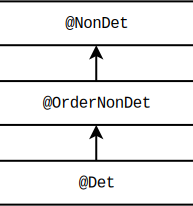
\includegraphics[scale=0.5]{determinism}
	\end{center}
	\caption{Determinism type hierarchy}
	\label{fig-determinism-hierarchy}
\end{figure}

In Figure~\ref{code-determinism}, we present some of the JDK methods that we have annotated with our determinism types and give examples of
client code that would produce errors at compile time.
\begin{figure}
	\begin{verbatim}
	// Annotated JDK methods
	public class Random implements java.io.Serializable {
	    public @NonDet Random() {}
	}
	public class PrintStream extends FilterOutputStream 
	    implements Appendable, Closeable {
	    public void println(@Det Object x) {}
	}
	
	// Client code
	class Client {
	    void test() {
	        @NonDet Random rnd = new Random(); // No error.
	        System.out.println(rnd);                    // Error - println takes @Det arguments.
	        @Det Random rnd1 = new Random();  // Error - subtyping rules violated.
	    }
	}
	\end{verbatim}
	\caption{Example: Errors detected by determinism checker}
	\label{code-determinism}
\end{figure}

\subsection{Determinism}

The underlying checker-framework on which we build our determinism checker has support for
polymorphic annotations. When a user writes a polymorphic annotation on a method signature or a type parameter,
it indicates that it could resolve to any type in the type system depending on how it is used.
In the determinism checker, we define a polymorphic annotation \<@PolyDet>.
One of the most common locations for a polymorphic annotation is at a method signature.
Consider the following method declaration annotated with polymorphic annotations
\begin{verbatim}
@PolyDet int foo(@PolyDet String param1, @PolyDet boolean param2) { }
\end{verbatim}
This indicates that method \<foo> can be called with arguments having any of the \codeid{@Det or @NonDet} type annotations 
(\<@OrderNonDet> is not allowed because it is invalid on primitive types). \<@PolyDet> resolves to the least upper bound of
the actual types on arguments. For instance, if this method is called as \codeid{foo(@Det String arg1, @NonDet boolean arg2)}, the 
checker framework resolves the method declaration as \codeid{@NonDet int foo(@NonDet String param1, @NonDet boolean param2)}
causing the return type to have the type annotation \<@NonDet>.


\subsection{Additional typing rules for collection elements}
The (determinism) type of a Collection or Iterator must be a supertype or equal to
the type of the type parameter (see Figure~\ref{fig-determinism-collections}).
If the Collection is \<@NonDet>, then the type parameter may not be
\<@Det> or \<@OrderNonDet>. Although such types could exist, they are
disallowed to prevent the following bug:

\begin{verbatim}
public static void add(@NonDet List<@Det String> list, @NonDet int index, @Det String s) {
    list.add(index, s);
}

public static void f(@Det List<@Det String> list, @NonDet int index, @Det String s) {
    add(list, index, s);
}
\end{verbatim}

The possibility of mutation allows us to add to the \<@Det List> at a
\<@NonDet> index, which is unsound.

Some examples of valid types are:
\begin{itemize}
	\item \codeid{@NonDet\ \ \ \ \ \ List<@NonDet\ \ \ \ \ \ Integer>}
	\item \codeid{@Det\ \ \ \ \ \ \ \ \ List<@Det\ \ \ \ \ \ \ \ \ Integer>}
	\item \codeid{@OrderNonDet Set <@OrderNonDet Set<...>\relax >}
	\item \codeid{@OrderNonDet Set <@Det String>}
	\item \codeid{@Det\ \ \ \ \ \ \ \ \ Map <@Det String, @Det Integer>}
	\item \codeid{@NonDet\ \ \ \ \ \ Set <T extends @NonDet Object>}
\end{itemize}

These types are invalid:
\begin{itemize}
	\item \codeid{@OrderNonDet Set <@NonDet\ \ \ \ \ \ Integer>}
	\item \codeid{@NonDet\ \ \ \ \ \ List<@Det\ \ \ \ \ \ \ \ \ Integer>}
	\item \codeid{@NonDet\ \ \ \ \ \ List<@OrderNonDet Set<...>\relax >}
	\item \codeid{@Det\ \ \ \ \ \ \ \ \ List<@NonDet\ \ \ \ \ \ Integer>}
	\item \codeid{@Det\ \ \ \ \ \ \ \ \ List<@OrderNonDet Set<...>\relax >}
	\item \codeid{@Det\ \ \ \ \ \ \ \ \ Map <@Det String, @OrderNonDet List<@Det String>>}
	\item \codeid{@Det\ \ \ \ \ \ \ \ \ List<T extends @NonDet Object>}
	\item \codeid{@NonDet\ \ \ \ \ \ Set\ <T extends @Det Object>}
\end{itemize}

Similarly, the (determinism) type of an array must be a supertype or equal to
the type of the component type (see Figure~\ref{fig-determinism-collections}).
As with collections, \codeid{@NonDet} arrays of \codeid{@Det} or \codeid{@OrderNonDet}
elements are not allowed.

For example, these types are valid:
\begin{itemize}
	\item \codeid{@NonDet int @NonDet \ \ \ \ []}
	\item \codeid{@Det \ \ \ int @Det \ \ \ \ \ \ \ []}
	\item \codeid{@Det \ \ \ int @OrderNonDet[] @OrderNonDet[]}
\end{itemize}

These types are invalid:
\begin{itemize}
	\item \codeid{@NonDet int @OrderNonDet[]}
	\item \codeid{@NonDet int @Det \ \ \ \ \ \ \ []}
	\item \codeid{@Det \ \ \ int @NonDet \ \ \ \ []}
\end{itemize}

\begin{figure}
	\centering
	\begin{tabular}{|l|l|l|l|l|}
		\cline{3-5}
		\multicolumn{2}{c|}{~}  &  \multicolumn{3}{c|}{Type Argument (or array component type)} \\ \cline{3-5}
		\multicolumn{2}{c|}{~}  & NonDet     & OrderNonDet & Det \\ \hline
		& NonDet      &   valid    &  invalid    & invalid  \\ \cline{2-5}
		Collection (or array)   & OrderNonDet &   invalid  &  valid      & valid  \\ \cline{2-5}
		& Det         &   invalid  &  invalid    & valid      \\ \hline
	\end{tabular}
	\caption{Valid Collection (and array) declarations.  The Collection's (or array's) type qualifier
		must be a supertype or equal to the type argument (or array component type).}
	\label{fig-determinism-collections}
\end{figure}

A collection (\<List, Set, or a Map>) annotated as \<@OrderNonDet> has the following properties:
\begin{enumerate}
	\item The individual elements extracted by iterating over the collection get the type \<@NonDet>.
	\item Accessing properties sich as \<size()> or querying if the collection \<isEmpty()> will return types
	that are annotated as \<@Det> as they do not depend on the iteration order. 
\end{enumerate}

A user defined type may be annotated as \<@OrderNonDet> if and only if it
is a subtype of Collection or Iterator.
For example, if a user defines a type as
\begin{verbatim}
public class TestUserCollection<E> extends ArrayList<E> {...}
\end{verbatim}
Writing \codeid{@OrderNonDet TestUserCollection<@Det Integer>} is valid.\\
Writing \codeid{@OrderNonDet TestUserCollection<@NonDet Integer>} is invalid
because the type of the type parameter (\codeid{@NonDet}) is not a subtype
of the user defined Collection type (\codeid{@OrderNonDet}).

User defined types that are not a subtype of Collection or Iterator
may not be annotated as \codeid{@OrderNonDet}.

\subsection{Polymorphism extensions}

Recall that the determinism checker does not permit \<@OrderNonDet> on a type that isn't a collection, iterator, or an array.
As a consequence, resolution of polymorphic type annotations at method signatures could have undesirable effects.
Suppose a method declaration is annotated as \codeid{@PolyDet int size(@PolyDet List<T> list)}. Invoking this method
as \codeid{size(@OrderNonDet List<@Det String>)} will result in \<@PolyDet> getting resolved to \<@OrderNonDet> which is invalid
on the return type \<int>. We circumvent this scenario by introducing two variants to the \<@PolyDet> annotation, \<@PolyDet("up")>
and \<@PolyDet("down")>. The semantics of these variants are as follows:
\begin{itemize}
	\item \<@PolyDet("up")>: Same as \<@PolyDet> except when it resolves to \<@OrderNonDet>, it is replaced with \<@NonDet>.
	\item \<@PolyDet("down")>: Same as \<@PolyDet> except when it resolves to \<@OrderNonDet>, it is replaced with \<@Det>.
\end{itemize} 
The modifiers "up" and "down" are indicative of the subtyping relationship of \<@OrderNonDet> with \<@NonDet> and \<@Det> respectively
in the determinism type hierarchy.
Annotating \<size()> as \codeid{@PolyDet("down") int size(@PolyDet List<T> list)} will only allow the following type resolutions:
\begin{itemize}
	\item \codeid{@Det int size(@Det List<T> list)}
	\item \codeid{@Det int size(@OrderNonDet List<T> list)}
	\item \codeid{@NonDet int size(@NonDet List<T> list)}
\end{itemize}

\subsection{Differentiating binding and use}

In order to provide soundness guarantees, we must ensure that a collection that is
declared as \<@Det> is not side-effected in non-deterministic ways. Consider the following annotation 
on the List add method: \codeid{public void add(@PolyDet ArrayList<E> this, @PolyDet int index, E element)}.
Suppose a client calls this method as follows:
\begin{verbatim}
@Det ArrayList<@Det String> list;
@NonDet int random;
@Det String str;
list.add(random, str);
\end{verbatim}
This will result in the instantion \codeid{public void add(@NonDet ArrayList<E> this, @NonDet int index, E element)} and
the method invocation will type check. This is problematic because even though \<list> was declared to be \<@Det>,
the type checker allows the addition of an element at a \<@NonDet> location violating our determinism guarantees.
We prevent this behavior by introducing another valiant of \<@PolyDet>, \<@PolyDet("use")> that does not affect
type instantiations. This is especially useful in preventing methods from non-deterministically modifying the state
of a deterministic receiver. To have this effect, the library method \<ArrayList.add> is annotated as:
\codeid{public void add(@PolyDet ArrayList<E> this, @PolyDet("use") int index, E element)}.
Since \<@PolyDet("use")> has no effect on type instantiations, calling this method on a \<@Det List>
will result in the method declaration being resolved as \codeid{public void add(@Det ArrayList<E> this, @Det int index, E element)}
irrespective of the type of \<index>, thereby preventing undesired side-effects.

\subsection{Dataflow analysis and type refinement}
The checker framework performs automatic type inference for local types within method bodies.
It also performs dataflow analysis and refines the types of these locals, thereby reducing the annotation burden 
on the programmer. Consider the example below:
\begin{verbatim}
void foo(@Det int x) {
    @NonDet int y = x;    // Type of y gets refined to @Det.
    @Det int z = y;       //  No error here.
}
\end{verbatim}
The checker framework performs dataflow analysis within method bodies and refines the types of local variables.
In the example above, even though the local variable \codeid{y} was declared to be \codeid{@NonDet}, it gets
type refined to \codeid{@Det} after the first assignment statement. As the result, the assignment of \codeid{y}
to a \codeid{@Det} variable \codeid{z} is sound. In the follwing example,
\begin{verbatim}
void foo(@NonDet Object x, @Det Object y) {
    x = y;                // No type refinement for x.
    @Det Object z = x;    // Error.
}
\end{verbatim}
the checker reports a warning at the second assignment statement of \codeid{foo}. Type refinement only applies to locals. Refining non-locals can result in side effects making the analysis unsound.

The determinism checker has additional type refinement rules for the sorting methods in collections. 
The checker type refines a receiver of type \codeid{@OrderNonDet List} to a \codeid{@Det List} if all the
type argument of this \codeid{List} have the type annotation \codeid{@Det}. Similar rules apply for \codeid{Arrays.sort()} and
\codeid{Collections.sort()}.
Under this if \codeid{sort()} is called on a receiver of type \codeid{@OrderNonDet List<@Det Set<@Det String>>}, it will
be type refined to \codeid{@Det List<@Det Set<@Det String>>}. However a receiver of type \codeid{@OrderNonDet List<@OrderNonDet Set<@Det String>>} will not be type refined.

\subsubsection{CLIMB-to-top and collection, array locals}

\begin{itemize}
	\item Every type system has a default annotation - the type that will be applied to unannotated locations.
	\item CF defaults types at CLIMB locations to top and type refines them. (steal some text from manual).
	\item CLIMB locations do not include type parameters. So this is problematic for determinism checker
	\item Example: Unannotated collection; its default would be \codeid{@NonDet<@Det>} which is invalid.
	\item So we default locals collections to \codeid{@NonDet<@NonDet>}. 
	\item This is sound but could produce a lot of FPs. Example assignment: \codeid{@NonDet<@NonDet> collection = collection1}.
	Type of collection1 is \codeid{@Det<@Det>} and it is a method argument.
	\item To avoid this, we require users to explicitly annotate local collections.
	\item Similarly for local arrays.
\end{itemize}

\subsection{Discussion on defaulting rules}

\begin{itemize}
	\item Determinism checker has \<@Det> as the usual default. Reason being we expect the program to be 
	deterministic unless specified by programmer or nondeterminism from libraries that we have annotated (Random, Collections, etc).
	\item All method parameters and return types (including constructors) are \<@PolyDet>.
	\item Reason: We want to be able to report nondeterministic behavior only where it is invalid.
	\item Example of a method with params and return types annotated as \<@PolyDet>.
	This method called from 2 places - one harmless(@Det instantiations), and another that call with \<@NonDet> args and prints the retun type.
	\item Exception to this defaulting is the construction of HashSets and HashMaps because they can't be \<@Det>.
	We explicitly annotate the return type on constructors as
        \<@OrderNonDet> and disallow constructing \<@Det HashSet> or \<@Det
        HashMap>.
\end{itemize}

\subsection{Additional hardcoded rules in the determinism checker  for precision}

\begin{itemize}
	\item \<Set.equals()> is annotated as \<@Poly("up")>. This is sound but imprecise.
	\item Example1: \codeid{@OrderNonDet Set<@Det List>.equals(@OrderNonDet Set<@Det List>)} is deterministic
	\item Example2: \codeid{@OrderNonDet Set<@OrderNonDet List>.equals(@OrderNonDet Set<@OrderNonDet List>)} is not deterministic.
	\item Explain the rules under which we make Set equality deterministic.
	\item We annotate System.getProperty as \<@NonDet> because the results could vary across machines.
	\item Exceptions: line.Sepaator, file.Separator. and path.Separator.
\end{itemize}

\subsection{Maps discussion}

\begin{itemize}
	\item A map is deterministic iff the \<entrySet()> is
          deterministic; equivalently, iff the \<keySet()> and \<values()>
          are both deterministic
	\item the iteration order of a keyset is the same as the iteration order of entrySet and Values.
	\item \<HashMap> - can be \<@OrderNonDet> or \<@NonDet>.
	\item \<LinkedHashMap> - can be \<@Det>, \<@OrderNonDet>, ot \<@NonDet>.
	\item \<TreeMap> - can be \<@Det> or \<@NonDet>.
	\item Problem with \<Map.get()> : Annotating as \<@PolyDet> is imprecise.
	\item We circumvent this by hardcoding rules to make it precise. (Describe the rule here)
	\item It was probably a bad design choice to make HashMap a subclass of Map (talk about how
	every method is overriden). Similarly for HashSet.
\end{itemize}

\subsection{Annotating more classes/providing more specifications}
\begin{itemize}
	\item Type system developer has to annotate methods in the JDK or any other library.
	\item Note: Another source of Nondeterminism we haven't analyzed: File system.
	\item Users can also provide stubs instead. (Steal some text from manual here)
\end{itemize}
